\documentclass[a4paper, 11pt]{article}
\usepackage{graphicx}
\usepackage{amsmath}
\usepackage[pdftex]{hyperref}

% Lengths and indenting
\setlength{\textwidth}{16.5cm}
\setlength{\marginparwidth}{1.5cm}
\setlength{\parindent}{0cm}
\setlength{\parskip}{0.15cm}
\setlength{\textheight}{22cm}
\setlength{\oddsidemargin}{0cm}
\setlength{\evensidemargin}{\oddsidemargin}
\setlength{\topmargin}{0cm}
\setlength{\headheight}{0cm}
\setlength{\headsep}{0cm}

\renewcommand{\familydefault}{\sfdefault}

\title{Data Mining: Learning from Large Data Sets - Fall Semester 2015}
\author{Lukasstr@ethz.ch\\ buehlmic@student.ethz.ch\\ habichta@student.ethz.ch\\}
\date{\today}

\begin{document}
\maketitle

\section*{Approximate near-duplicate search using Locality Sensitive Hashing} 


The implementation follows a \textit{Min-hashing} approach as a locality sensitive hashing scheme. The main bulk of the implementation focuses on creating a \textit{signature matrix} $M$.  In each row, $M$ contains the minimum indices of non-zero column values, found in the row-wise permuted \textit{shingle matrix} $S$. $S$ is permuted several times by defining a linear hash function $\pi(r)$, which is defined as follows.
$$ \pi_{i}(r) =  a_{i}r + b \bmod n$$
The function describes the $i$-th permutation of a row $r$ of the matrix $S$. The exact permutation of all rows is determined by the randomly generated values $a_{i}$ and $b$. In order to reduce the number of hash collisions, $n$ signifies a  prime number. The function $h_{\pi_{i}}(C)$ is then applied to each permutation of $S$.
$$h_{\pi_{i}}(C)  = \min_{r:C(r)=1} \pi_{i}(r)$$
Applied to each input document (video), this creates the $i$-th row of $M$. According to the law of large numbers, the (row-wise) similarity of the columns in M will converge to the \textit{Jaccard similarity}. Increasing the number of permutations (hash functions) decreases the rate of false negatives. However, it also increases the number of false positives. Therefore, this implementation uses a composition of r-way AND and b-way OR hash functions. $M$ is partitioned into $b$ bands with $r$ rows each. Each band $j$ hashes its columns to a specific value, called a $bucket$. For each band, we apply $h(s)$

$$h(s) = \displaystyle\sum_{i=1}^{r} a_{i}s_{i} + b \bmod n $$

$s$ is a vector of size r, containing the values of a column within a band. The other parameters have the same meaning as described above. However, different values are chosen. Videos, whose bands appear in the same bucket at least once are then further investigated. Their shingles are compared to derive the Jaccard similarity. If the similarity is at least 90\%, their identification numbers are outputted.

The implementation uses the \textit{MapReduce} paradigm to exploit the inherent parallelism found in the approach described above. \newline The \textit{Mapper} processes are responsible for creating $M$ and hashing the the bands into their respective buckets. At the beginning, they define the number of hash functions which can be derived by the multiplication of the \texttt{band\_size} ($r$) and the \texttt{num\_bands} ($b$). In this implementation, $r$ amounts to 25 and $b$ is 39. Consequently, the number of hash functions is 975 for the signature matrix plus 39 for the hash bands. Hence we have 975 + 39 = 1014 hash functions in total. This performs quite well and gives us only a very small amount of False-Negatives (see Figure \ref{perfPlot}). (Remark: In our latest version we fixed \texttt{band\_size} = 16 and \texttt{num\_bands} = 60. With that we got a score of 1.0.)
\begin{figure}
	\begin{center}
		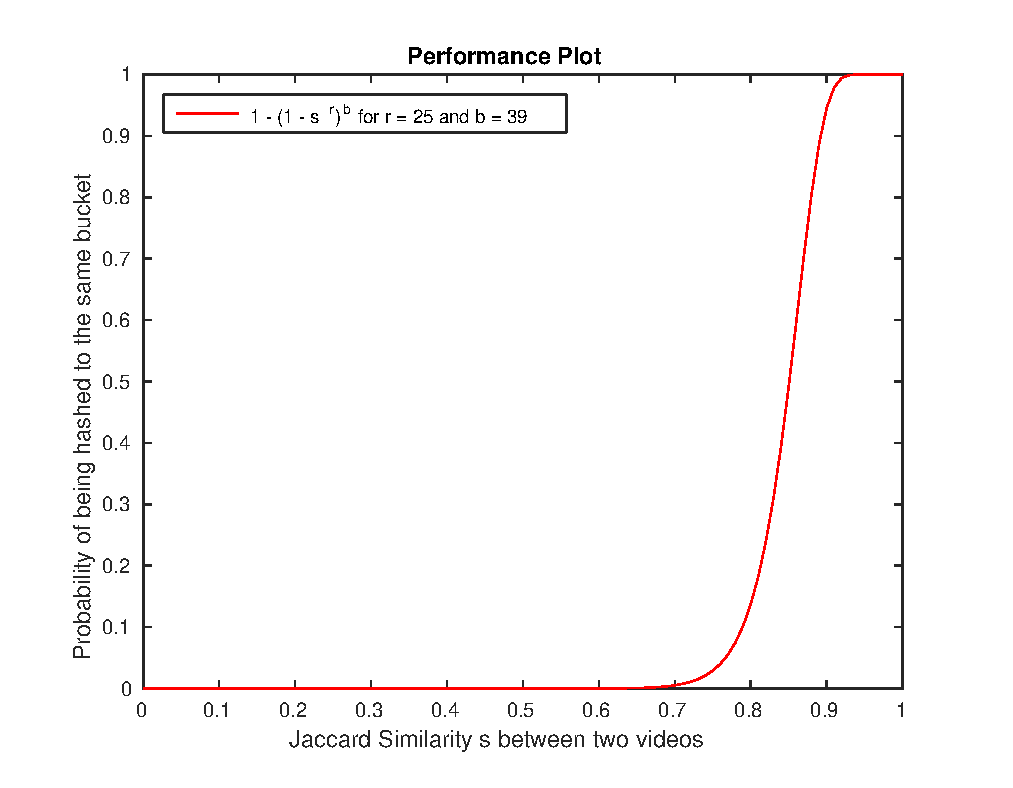
\includegraphics[scale=0.4]{performance}
		\caption{Plots the probability that two videos are being hashed to the same bucket against the Jaccard Similarity of the two videos.}
		\label{perfPlot}
	\end{center}
\end{figure}

Furthermore, the \texttt{numpy} library is used to generate random values for the calculations outlined above. The Mapper receives the \texttt{video\_id} and the corresponding  \texttt{shingles}. It then constructs one column of the signature matrix of that video by calling \texttt{construct\_column\_from\_shingles()}. It uses a matrix initialized with a value larger than the largest possible shingle value. Since the shingle value concurs with the non-zero indices of $S$ (one column per video), finding the minimum shingle value after permuting the rows of the column is equivalent to finding the smallest non-zero index. This is done iteratively. The function loops over each shingle and row of $M$ (this is the same as iterating over each hash function), does a linear hash, and finds the minimum for each row. This yields a full column of $M$. \newline 
Afterwards, it defines the bands with \texttt{hash\_bands()}. It calculates the buckets in which each band of the column is mapped and returns a map \texttt{hash\_values} to save this mapping. The Mapper then returns  strings of the form ``\texttt{\%s \%s\textbackslash t\%s \%s}''. The first value is the \texttt{band\_number} and the second the \texttt{hash\_values[band\_number]}. The letter signifies the bucket number in which the respective band was hashed. Both values form the key that is later used by the reducer. The remaining values are the \texttt{video\_id} and the sorted \texttt{shingles}.

The \texttt{Reducer} processes receive the Mapper's outputs in a sorted manner (sorted by the key).  The Reducer first parses the input and checks if a specific key was seen before. If this is the case, then a possible duplicate is detected (the same bands of different videos are hashed into the same bucket). The possible duplicates are saved in a set. As soon as a new key appears, this set is evaluated by the \texttt{print\_duplicates()} function. This function compares all the possible duplicates with each other by calculating the Jaccard similarity of all their shingles. if it is larger or equal to 90\%, it prints both \texttt{video\_ids} in ascending order.


\end{document} 
